\documentclass[xcolor=dvipsnames, 12pt, handout]{beamer}
\useoutertheme{infolines} 
%\definecolor{grayish}{RGB}{147,162,153}
\usecolortheme[named=gray]{structure} 
\usetheme[height=7mm]{Rochester}

\usepackage{graphicx}

\usepackage{AMMALanguages}
\usepackage{hyperref}
\usepackage{tikz}
\usetikzlibrary{positioning}
\usetikzlibrary{arrows,shapes}

%\setbeameroption{show notes}
%\setbeameroption{show only notes}
\setbeamertemplate{note page}[plain]

\usepackage[utf8]{inputenc}
\usepackage[T1]{fontenc}

\usepackage{listings}

\newcommand\blfootnote[1]{%
  \begingroup
  \renewcommand\thefootnote{}\footnote{#1}%
  \addtocounter{footnote}{-1}%
  \endgroup
}

\AtBeginSection{\frame{\sectionpage}}

\title[SyVOLT]{SyVOLT: Full Model Transformation Verification Using Contracts}
%\title{Full Verification of Model Transformation Contracts for Declarative ATL}
\author[Lucio, Oakes]{Levi L\'{u}cio, \textbf{Bentley James Oakes}}
%\subtitle{}
%\logo{}
\institute[]{McGill University, Canada\\fortiss, Munich}
%\date{}
%\subject{}
%\setbeamercovered{transparent}
%\setbeamertemplate{navigation symbols}{}

% logo of my university
%\titlegraphic{\vspace{-0.5cm}
\includegraphics[width=3cm]{figures/mcgill}\hspace*{4.75cm}~%
%   
\includegraphics[width=4cm]{figures/big}
%}

\begin{document}
\maketitle

%\section{Intro}

\begin{frame}{Motivation and Overview}
\begin{itemize}[<+->]
\item Model transformations are at the heart of model-driven engineering
\item Want to verify correctness for transformation specifications
\begin{itemize}[<+->]
\item Verify visual/structural contracts
\item Identify those combinations of rules where contracts hold or not
\end{itemize}
\item Objective: Verification for all input models
\begin{itemize}
\item Input independence
\end{itemize}
\end{itemize}
\end{frame}


%\section{Families-To-Persons Transformation}




\begin{frame}{DSLTrans Transformation}

\begin{itemize}[<+->]
\item Visual language for model transformations

\item Graph-based, rule-based
\item Out-place so no rewriting performed
\begin{itemize}
\item Suited for `translation' transformations
\end{itemize}
\item All its computations are terminating and confluent
\item Unbounded loops during execution are not allowed

\item Rules are grouped in sequential layers
\end{itemize}

\blfootnote{Selim, Gehan et al. "Model transformations for migrating legacy deployment models in the automotive industry." Software and Systems Modeling 14, no. 1 (2013): 365-381.}

\end{frame}


\begin{frame}{Transformation Metamodels}

\begin{center}
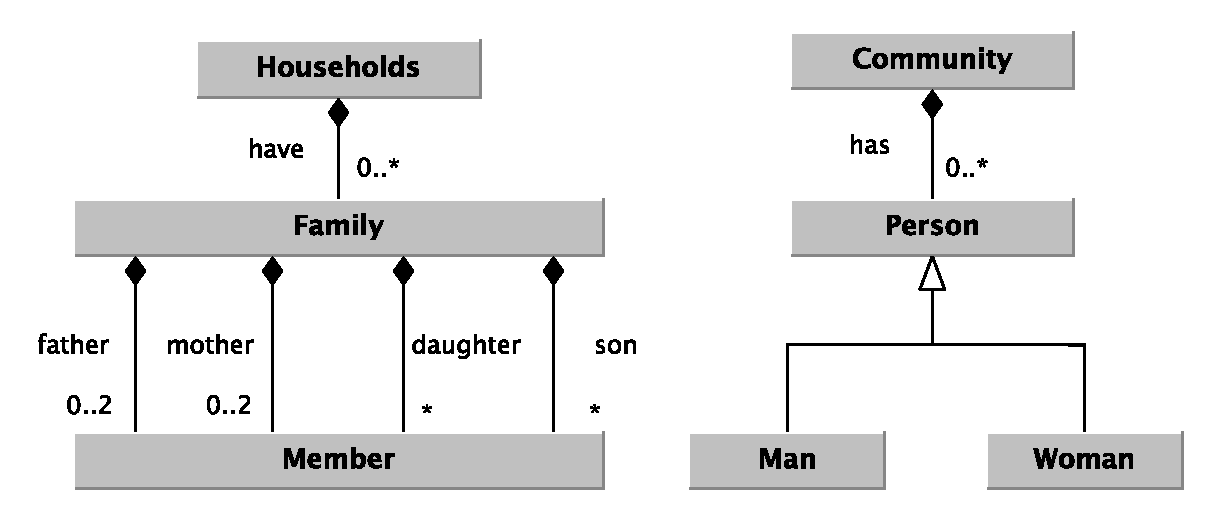
\includegraphics[width=0.8\textwidth]{figures/Metamodels_F2P}
\end{center}
\begin{itemize}
\item Transform \textit{Members} to \textit{Men} and \textit{Women}
\end{itemize}
\end{frame}


\begin{frame}{DSLTrans}
\begin{center}
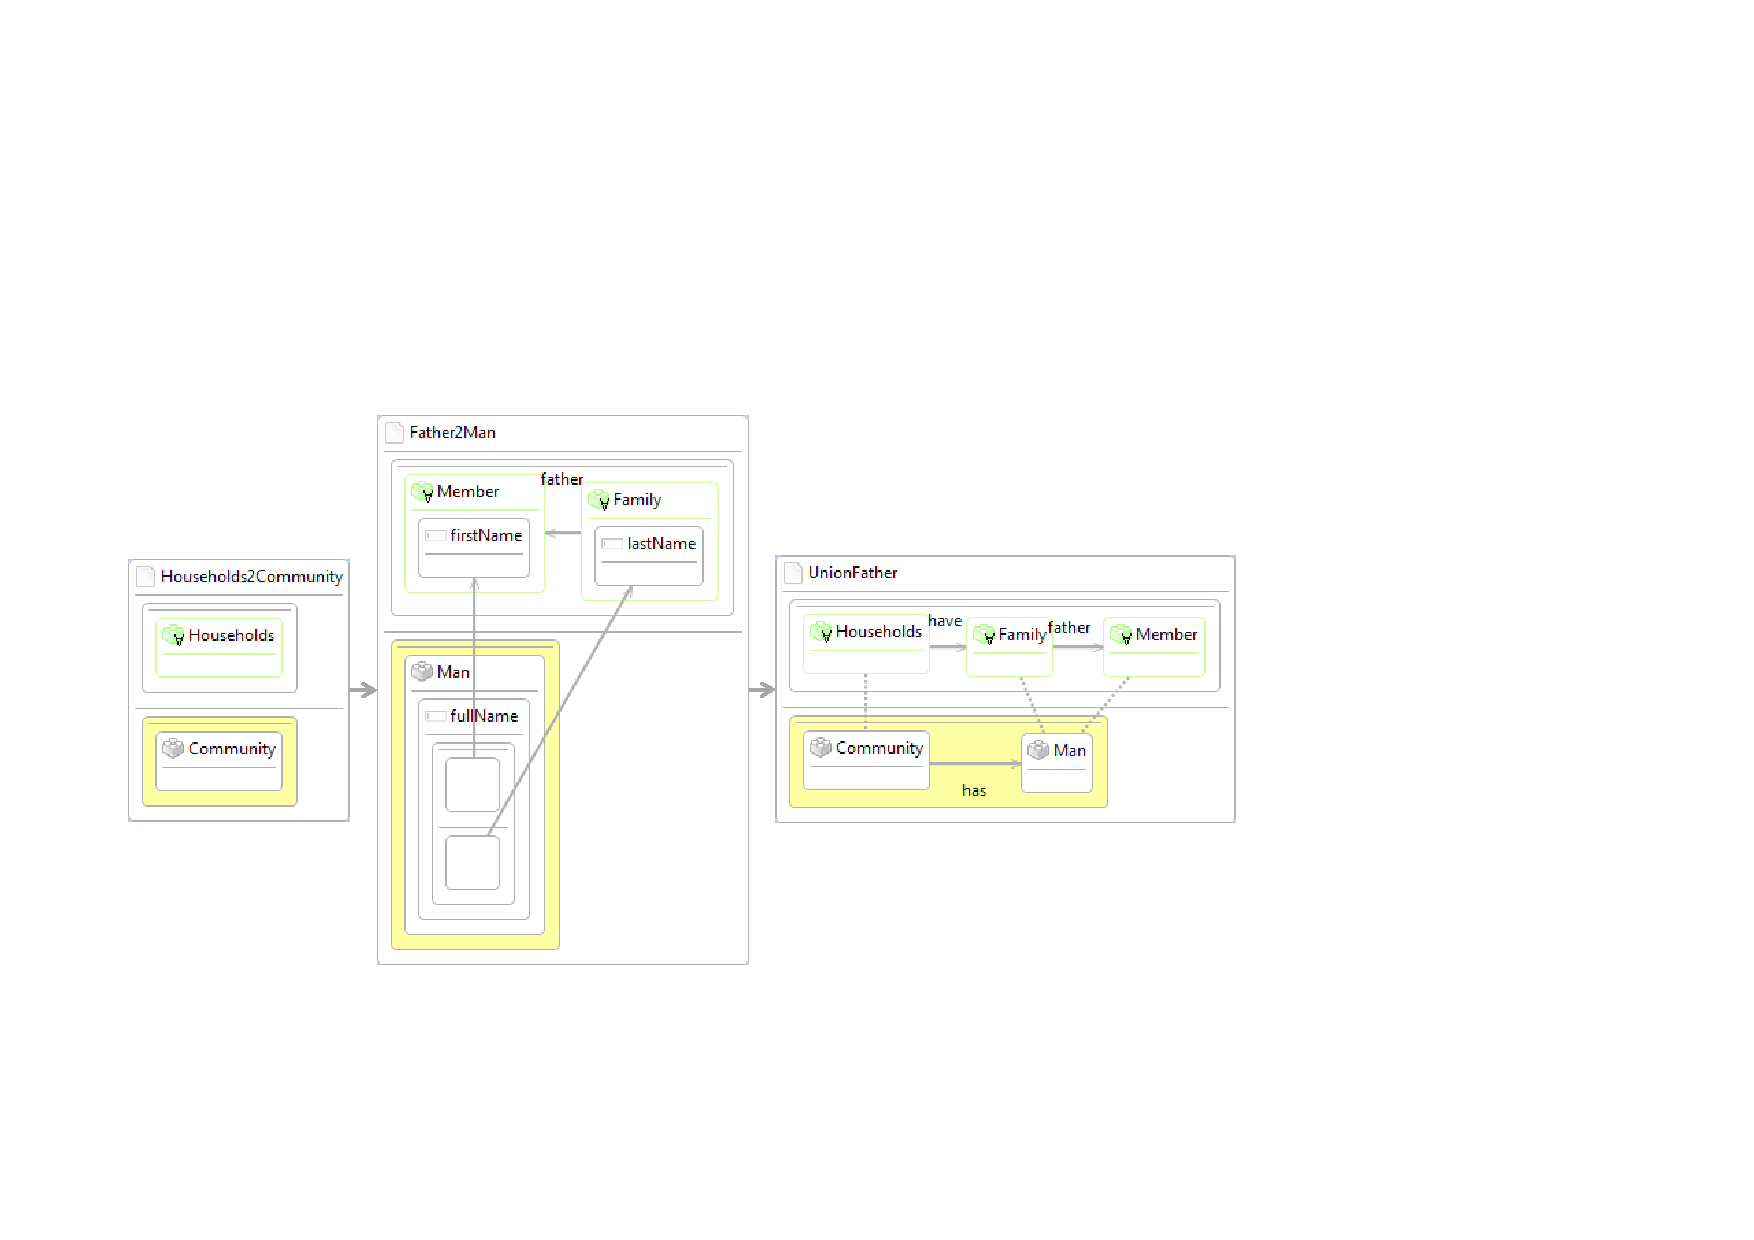
\includegraphics[width=\textwidth]{figures/Rules}
\end{center}
\pause
\begin{itemize}[<+->]
\item Rules arranged in layers
\item Match graph on top of rules
\item Apply graph on bottom
\begin{itemize}
\item Produced when match graph is found
\end{itemize}
\end{itemize}
\end{frame}




\begin{frame}{Pre- / Post- Visual Contracts}
\begin{center}
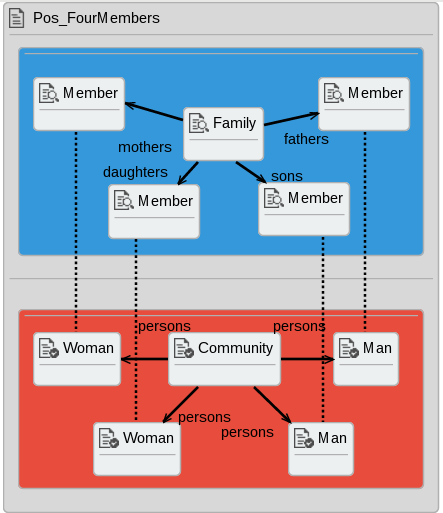
\includegraphics[width=0.35\textwidth]{figures/Pos_FourMembers}
\end{center}
\pause
\begin{itemize}[<+->]
\item If blue graph is found in input model, then red graph is found in output model
\item Objective: Prove for all input models/transformation executions - input independence
\item \textit{A family with a father, mother, son, daughter
should always produce two males and two females in the
target community}
\end{itemize}
\end{frame}

\begin{frame}{SyVOLT Tool}
\begin{itemize}[<+->]
\item Proves contracts on DSLTrans transformations
\item All possible executions of the transformation are symbolically constructed
\begin{itemize}[<+->]
\item Built as sets of rules called path conditions
\begin{itemize}
\item No rules execute, only rule 1 executes, rule 1 and rule 2 both execute
\item Rule dependencies/combinations resolved
\end{itemize}
\item Final finite set of path conditions represents all possible transformation executions
\end{itemize}
\item A contract holds for a transformation if it holds for all generated path conditions
\item Otherwise, counter-example is produced
\end{itemize}
\blfootnote{L. Lúcio, B. Oakes, and H. Vangheluwe. A technique for symbolically verifying properties of graph-based model transformations. Technical report, Technical Report SOCS-TR-2014.1, McGill U, 2014.}
\end{frame}

\begin{frame}{Contract Proving Example}
\begin{center}
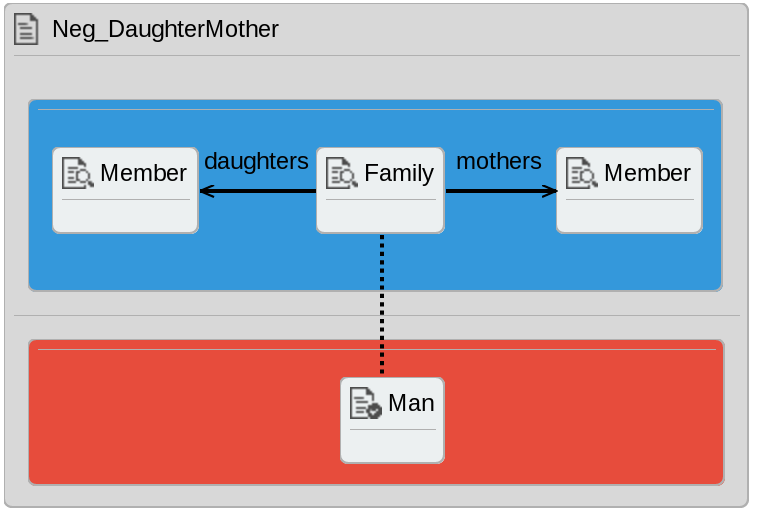
\includegraphics[width=0.7\textwidth]{figures/Pos_DaughterMother}
\end{center}
\begin{itemize}[<+->]
\item Statement: \textit{A family with a mother and a daughter will always produce a community with a man}
\item Fails on path condition: `HFamComm\_HMotherRule\_HDaughterRule'
\end{itemize}
\end{frame}


\begin{frame}{Performance}
\begin{center}
\setlength\tabcolsep{3pt}  % default value: 6pt
\tiny  %%  command to change the font size

\begin{tabular}{l | c| | r |r || r |r || r}
 &  \textbf{ATL/ DSLTrans}&  \textbf{Path Conds.}  & \textbf{Time (s)} & \textbf{Contracts} & \textbf{Time (s)}& \textbf{Memory}\\
 & \centering \textbf{Rules}&  \textbf{Generated}&  &  \textbf{Proved}& & \textbf{(MB)} \\ \hline\hline
Families-to-Person & \centering 5 / 9 & 101 & \textbf{0.24} & 4 & \textbf{0.52}& 54\\\hline
Ext. Families-to-Person & \centering10  / 19 & 366	& \textbf{3.89} & 10	& \textbf{7.35} & 59\\\hline
GM-to-AUTOSAR (handbuilt)& \centering5 / 9 & 13 & \textbf{0.18} & 9 &\textbf{ 0.15 }& 58\\
GM-to-AUTOSAR (HOT)& \centering5 / 9 & 10 & \textbf{0.26} & 9 & \textbf{0.15} & 60\\\hline
UML-to-Kiltera & \centering20 / 17 & 322 & \textbf{1.86} & 15 & \textbf{11.99} & 55\\
\end{tabular}
\end{center}
\begin{itemize}
\item Multiple contracts can be proved in seconds
\end{itemize}
\end{frame}

\begin{frame}{Contract Expressibility}

\begin{itemize}[<+->]
\item Next few slides will discuss concepts expressible with our contract language.

\begin{itemize}[<+->]
\item Pattern contracts
\item Element attributes
\item Propositional logic and pivots
\item Syntactic invariants
\item Multiplicity invariants
\end{itemize}
\end{itemize}

\begin{itemize}
\item Rule reachability is also handled by the prover, which reports if a rule cannot be proven to execute
\end{itemize}

\blfootnote{Selim, G.M.: Formal Verification of Graph-Based Model Transformations. Ph.D. thesis, Queen’s University. 2015.}
\end{frame}

\begin{frame}{Pattern Contracts}
\begin{center}
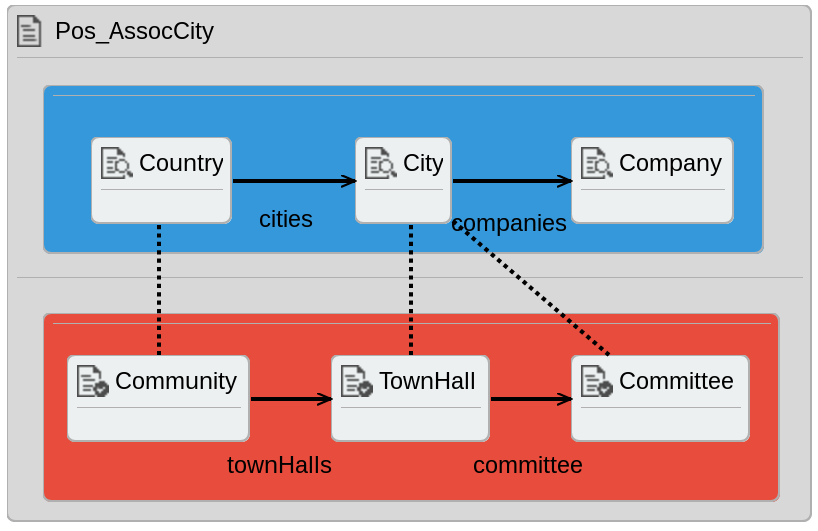
\includegraphics[width=0.7\textwidth]{figures/Pos_AssocCity}
\end{center}
\begin{itemize}
\item Relates elements in input model to elements in output model
\item \textit{A country which contains a city, which contains a company, produces a corresponding community, town hall, and committee}
\item Intention is to allow verification that multiple rules are interacting in a valid way
\begin{itemize}
\item Difficult from manual inspection of the rules themselves
\end{itemize}
\end{itemize}
\end{frame}


\begin{frame}{Element Attributes}
\begin{center}
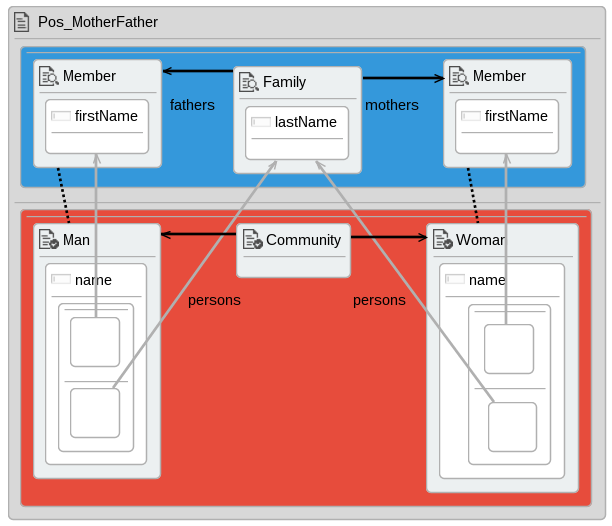
\includegraphics[width=0.50\textwidth]{figures/Pos_MotherFather}
\end{center}
\pause
\begin{itemize}[<+->]
\item Reasoning about (String) attributes of elements
\item \textit{Is the full name of the produced Person correctly created from the last name of the Family and the first name of the Member?}
\end{itemize}
\end{frame}

\begin{frame}{Propositional Logic and Pivots}
\begin{center}
\begin{center}
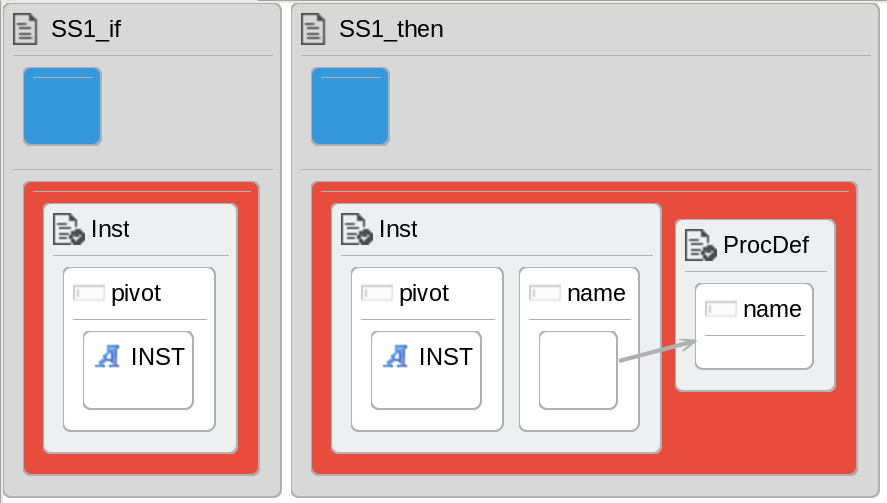
\includegraphics[width=0.45\textwidth]{figures/syntactic_invariant}
\end{center}
\end{center}
\pause
\begin{itemize}[<+->]
\item Contracts can be combined with AND, OR, NOT, IF-THEN
\item Pivots ensure that same element is bound in both contracts
\item \textit{Only one Person is in the Community in the output model}
\end{itemize}
\end{frame}

\begin{frame}{Syntactic Invariants}
\begin{center}
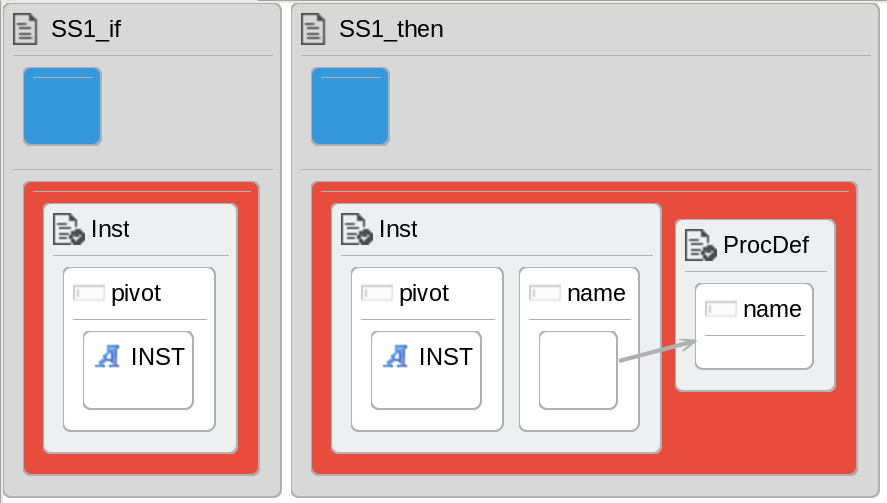
\includegraphics[width=0.7\textwidth]{figures/syntactic_invariant}
\end{center}
\begin{itemize}
\item Check if path condition is well-formed input or output syntax
\item \textit{If there is an Inst element, then that Inst element has the same name as a ProcDef element}
\end{itemize}
\end{frame}

\begin{frame}{Multiplicity Invariants}
\begin{center}
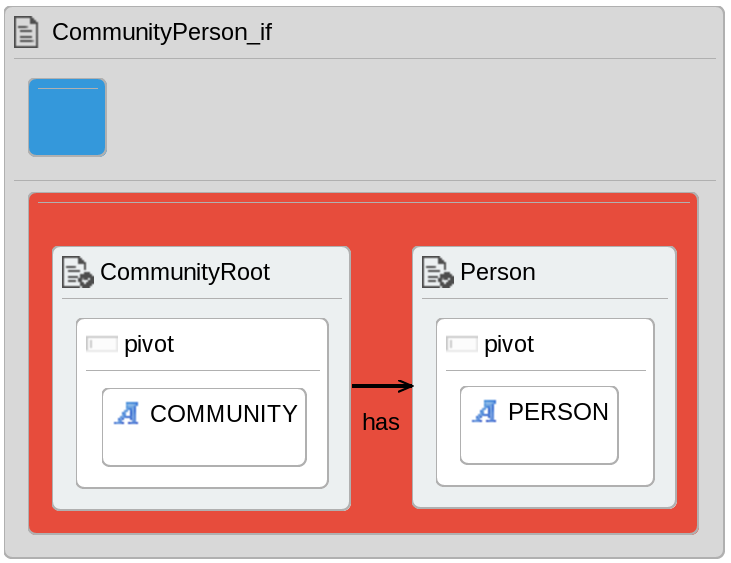
\includegraphics[width=0.45\textwidth]{figures/communityPersonProp_if}
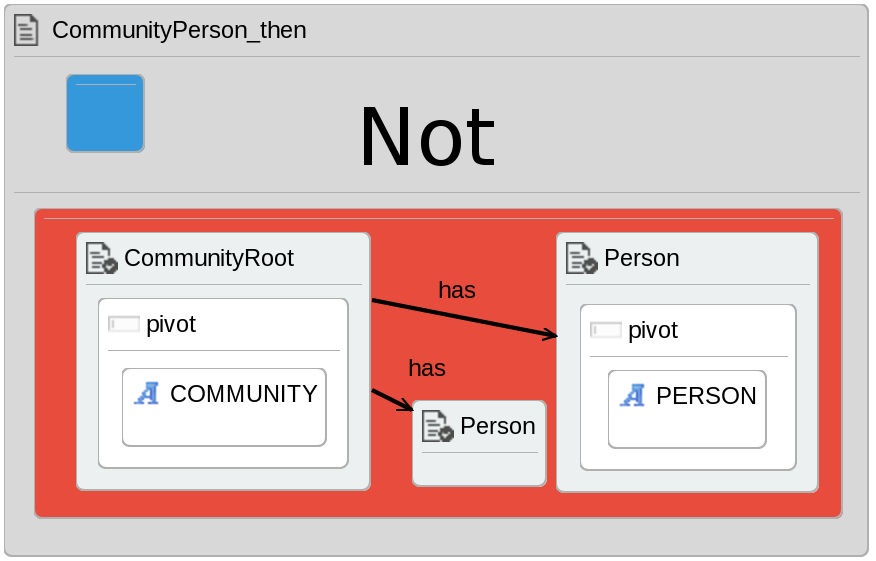
\includegraphics[width=0.45\textwidth]{figures/communityPersonProp_then}
\end{center}
\begin{itemize}
\item \textit{Only one Person is in the Community in the output model}
\end{itemize}
\begin{itemize}
\item Abstraction of our approach loses multiplicity information
\begin{itemize}
\item Multiple applications of a rule are not represented
\end{itemize}
\item Contract only fails if \textit{two Persons are always created in output}
\end{itemize}
\end{frame}



\begin{frame}{Contract Limitations}

\begin{itemize}
\item Limitations from symbolic execution technique
\begin{itemize}
\item Loses multiplicity information
\item Difficult to reason about negative contracts
\item Cannot validate instance data
\end{itemize}
\item DSLTrans transformation language only manipulates Strings
\begin{itemize}
\item Can be worked around
\end{itemize}
\end{itemize}
\end{frame}

\begin{frame}{Contract Limitations}

\begin{itemize}
\item Contract language equipped for structural queries
\begin{itemize}
\item Cannot compute queries
\end{itemize}
\item Abstractly representation of the rules that
execute, and the number of times each rule executes,
\item Cannot validate instance data for input or output models
\begin{itemize}
\item All input names start with a capital
letter.
\end{itemize}
\end{itemize}
\end{frame}


\begin{frame}{Current Work - mbeddr}

\begin{itemize}[<+->]
\item Verify contracts on the mbeddr  to C transformation
\item mbeddr takes components of embedded system expressed in MPS and generates C code
\item Transformation must be verified in order to ensure that resulting C code is valid
\end{itemize}
\end{frame}

\begin{frame}{Challenges}

\begin{center}
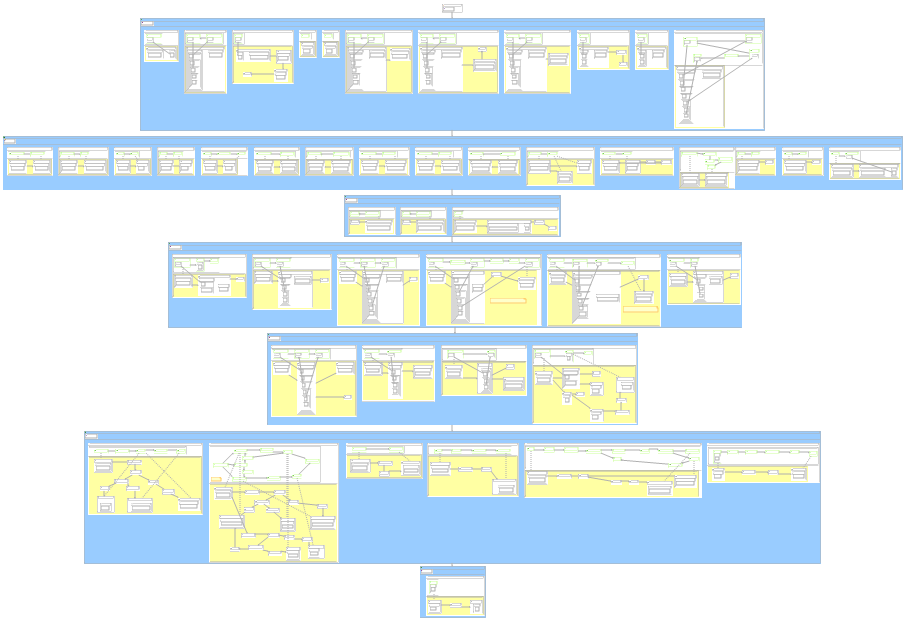
\includegraphics[width=0.7\textwidth]{figures/mbeddr}
\end{center}

\begin{itemize}
\item Scalability
\item What are appropriate contracts for this transformation?

\end{itemize}
\end{frame}

\begin{frame}{Other Work}
\small
\begin{itemize}[<+->]

\item Fully Verifying Transformation Contracts for Declarative ATL (MODELS 2015)\\

Bentley James Oakes, Javier Troya, Levi Lucio, and Manuel Wimmer\\
(McGill University, Canada; Vienna University of Technology, Austria)
\begin{itemize}
\item Extended to journal article: Full Contract Verification for ATL using Symbolic Execution, SoSym (to appear)
\end{itemize}
\item  Finding and fixing bugs in model transformations with formal verification: An experience report (AMT)\\
Gehan M. K. Selim, James R. Cordy, Juergen Dingel, Levi Lucio and Bentley James Oakes\\
(Queen's University, Canada; McGill University, Canada) 
\item 
\end{itemize}
\end{frame}

\begin{frame}{Eclipse Plugin}
\begin{center}
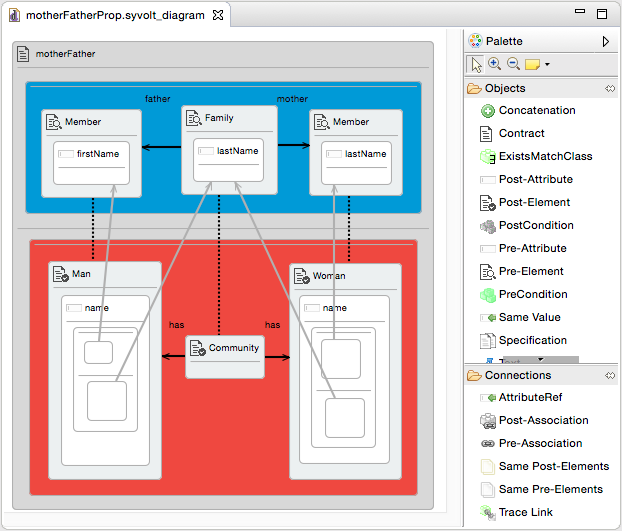
\includegraphics[width=\textwidth]{figures/eclipse_frontend}
\end{center}

\begin{itemize}
\item Eclipse Graphical Modeling Framework plugin
\item Allows for building of DSLTrans transformations and contracts.
\item Fully automatic proving process and the approach's formal details are completely hidden from the user.
\item Property proving process will automatically
            create all required artifacts, run
            the process, and provide the results to the user within the
            Eclipse environment.
\item User always stays within the Eclipse
            environment when developing the contracts and the model
            transformations.
\end{itemize}
\end{frame}

\begin{frame}{Conclusion}
\begin{itemize}[<+->]
\item Can verify visual contracts on DSLTrans transformations in feasible time
\item Contracts verified on all transformation executions
\item Eclipse plugin to build transformation and contracts
\item Future work is to focus on contract-driven development of model transformations
\end{itemize}
\pause
\begin{itemize}
\item Thank you for your time!
\end{itemize}
\begin{center}
\textbf{SyVOLT: Full Model Transformation Verification Using Contracts}\\
\end{center}
\end{frame}


\end{document}
